\documentclass[twoside]{book}

% Packages required by doxygen
\usepackage{fixltx2e}
\usepackage{calc}
\usepackage{doxygen}
\usepackage[export]{adjustbox} % also loads graphicx
\usepackage{graphicx}
\usepackage[utf8]{inputenc}
\usepackage{makeidx}
\usepackage{multicol}
\usepackage{multirow}
\PassOptionsToPackage{warn}{textcomp}
\usepackage{textcomp}
\usepackage[nointegrals]{wasysym}
\usepackage[table]{xcolor}

% Font selection
\usepackage[T1]{fontenc}
\usepackage[scaled=.90]{helvet}
\usepackage{courier}
\usepackage{amssymb}
\usepackage{sectsty}
\renewcommand{\familydefault}{\sfdefault}
\allsectionsfont{%
  \fontseries{bc}\selectfont%
  \color{darkgray}%
}
\renewcommand{\DoxyLabelFont}{%
  \fontseries{bc}\selectfont%
  \color{darkgray}%
}
\newcommand{\+}{\discretionary{\mbox{\scriptsize$\hookleftarrow$}}{}{}}

% Page & text layout
\usepackage{geometry}
\geometry{%
  a4paper,%
  top=2.5cm,%
  bottom=2.5cm,%
  left=2.5cm,%
  right=2.5cm%
}
\tolerance=750
\hfuzz=15pt
\hbadness=750
\setlength{\emergencystretch}{15pt}
\setlength{\parindent}{0cm}
\setlength{\parskip}{3ex plus 2ex minus 2ex}
\makeatletter
\renewcommand{\paragraph}{%
  \@startsection{paragraph}{4}{0ex}{-1.0ex}{1.0ex}{%
    \normalfont\normalsize\bfseries\SS@parafont%
  }%
}
\renewcommand{\subparagraph}{%
  \@startsection{subparagraph}{5}{0ex}{-1.0ex}{1.0ex}{%
    \normalfont\normalsize\bfseries\SS@subparafont%
  }%
}
\makeatother

% Headers & footers
\usepackage{fancyhdr}
\pagestyle{fancyplain}
\fancyhead[LE]{\fancyplain{}{\bfseries\thepage}}
\fancyhead[CE]{\fancyplain{}{}}
\fancyhead[RE]{\fancyplain{}{\bfseries\leftmark}}
\fancyhead[LO]{\fancyplain{}{\bfseries\rightmark}}
\fancyhead[CO]{\fancyplain{}{}}
\fancyhead[RO]{\fancyplain{}{\bfseries\thepage}}
\fancyfoot[LE]{\fancyplain{}{}}
\fancyfoot[CE]{\fancyplain{}{}}
\fancyfoot[RE]{\fancyplain{}{\bfseries\scriptsize Generated by Doxygen }}
\fancyfoot[LO]{\fancyplain{}{\bfseries\scriptsize Generated by Doxygen }}
\fancyfoot[CO]{\fancyplain{}{}}
\fancyfoot[RO]{\fancyplain{}{}}
\renewcommand{\footrulewidth}{0.4pt}
\renewcommand{\chaptermark}[1]{%
  \markboth{#1}{}%
}
\renewcommand{\sectionmark}[1]{%
  \markright{\thesection\ #1}%
}

% Indices & bibliography
\usepackage{natbib}
\usepackage[titles]{tocloft}
\setcounter{tocdepth}{3}
\setcounter{secnumdepth}{5}
\makeindex

% Custom commands
\newcommand{\clearemptydoublepage}{%
  \newpage{\pagestyle{empty}\cleardoublepage}%
}

\usepackage{caption}
\captionsetup{labelsep=space,justification=centering,font={bf},singlelinecheck=off,skip=4pt,position=top}

%===== C O N T E N T S =====

\begin{document}

% Titlepage & ToC
\pagenumbering{roman}
\begin{titlepage}
\vspace*{7cm}
\begin{center}%
{\Large A\+R\+Drone }\\
\vspace*{1cm}
{\large Generated by Doxygen 1.8.11}\\
\end{center}
\end{titlepage}
\clearemptydoublepage
\tableofcontents
\clearemptydoublepage
\pagenumbering{arabic}

%--- Begin generated contents ---
\chapter{Hierarchical Index}
\section{Class Hierarchy}
This inheritance list is sorted roughly, but not completely, alphabetically\+:\begin{DoxyCompactList}
\item Q\+Widget\begin{DoxyCompactList}
\item \contentsline{section}{keyboard\+\_\+controller}{\pageref{classkeyboard__controller}}{}
\end{DoxyCompactList}
\end{DoxyCompactList}

\chapter{Class Index}
\section{Class List}
Here are the classes, structs, unions and interfaces with brief descriptions\+:\begin{DoxyCompactList}
\item\contentsline{section}{{\bf keyboard\+\_\+controller} \\*Class to handle the keyboard controller }{\pageref{classkeyboard__controller}}{}
\end{DoxyCompactList}

\chapter{Class Documentation}
\section{keyboard\+\_\+controller Class Reference}
\label{classkeyboard__controller}\index{keyboard\+\_\+controller@{keyboard\+\_\+controller}}


Class to handle the keyboard controller.  




{\ttfamily \#include $<$ardrone\+\_\+test.\+h$>$}

Inheritance diagram for keyboard\+\_\+controller\+:\begin{figure}[H]
\begin{center}
\leavevmode
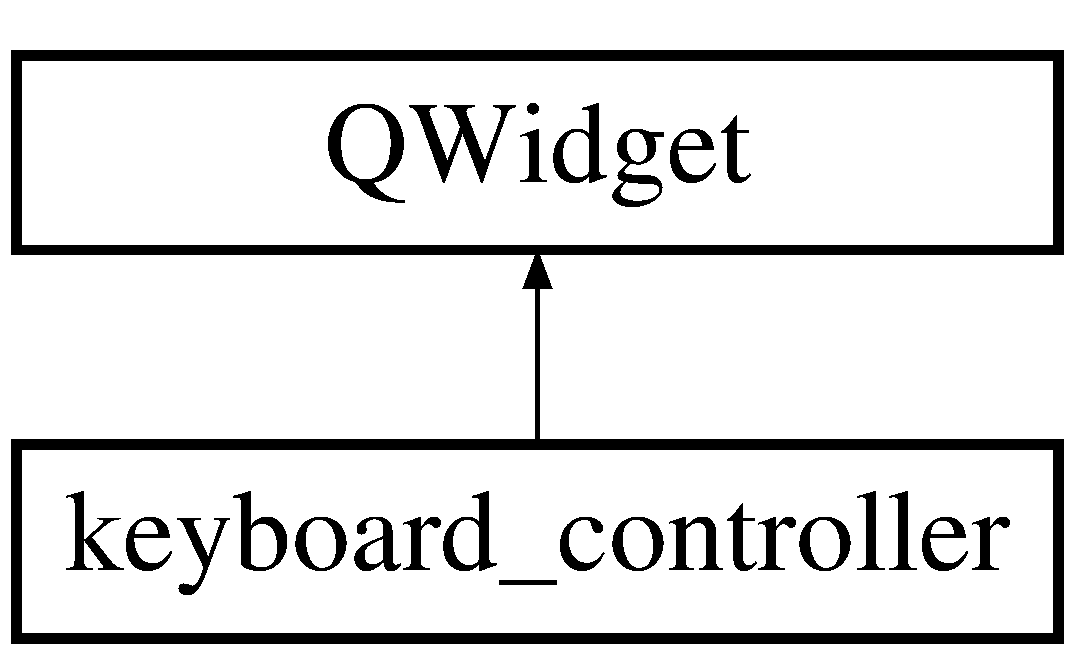
\includegraphics[height=2.000000cm]{classkeyboard__controller}
\end{center}
\end{figure}
\subsection*{Public Member Functions}
\begin{DoxyCompactItemize}
\item 
{\bf keyboard\+\_\+controller} (ros\+::\+Node\+Handle node)
\begin{DoxyCompactList}\small\item\em Constructor. \end{DoxyCompactList}\item 
{\bf $\sim$keyboard\+\_\+controller} (void)
\begin{DoxyCompactList}\small\item\em Destructor. \end{DoxyCompactList}\item 
void {\bf image\+Callback} (const sensor\+\_\+msgs\+::\+Image\+Const\+Ptr \&msg)
\begin{DoxyCompactList}\small\item\em Image Callback. \end{DoxyCompactList}\item 
void {\bf navdata\+Callback} (const ardrone\+\_\+autonomy\+::\+Navdata \&data)
\begin{DoxyCompactList}\small\item\em Navigation Data Callback. \end{DoxyCompactList}\end{DoxyCompactItemize}
\subsection*{Private Member Functions}
\begin{DoxyCompactItemize}
\item 
void {\bf key\+Press\+Event} (Q\+Key\+Event $\ast$e)
\begin{DoxyCompactList}\small\item\em Handle the Key Press Event. \end{DoxyCompactList}\item 
void {\bf key\+Release\+Event} (Q\+Key\+Event $\ast$key)
\begin{DoxyCompactList}\small\item\em Handle the Key Release Event. \end{DoxyCompactList}\end{DoxyCompactItemize}
\subsection*{Private Attributes}
\begin{DoxyCompactItemize}
\item 
int {\bfseries state}\label{classkeyboard__controller_a4296d4dabdd9bed06091159d968be284}

\item 
float {\bfseries velocity}\label{classkeyboard__controller_aa7b7cce2981ab1f4a067e455a4a44e38}

\item 
geometry\+\_\+msgs\+::\+Twist {\bfseries twist\+\_\+msg}\label{classkeyboard__controller_aa7ec9a03d00fdf4d2d4e751a55ecad0d}

\item 
std\+\_\+msgs\+::\+Empty {\bfseries emp\+\_\+msg}\label{classkeyboard__controller_aaa44aba2c4397ff6c1beb6c4b0c095a3}

\item 
ros\+::\+Publisher {\bfseries pub\+\_\+empty\+\_\+land}\label{classkeyboard__controller_acd15f5c9ecc27236e49c633b903b5065}

\item 
ros\+::\+Publisher {\bfseries pub\+\_\+twist}\label{classkeyboard__controller_ad95754cc2758fb39abdf235d4ca93d67}

\item 
ros\+::\+Publisher {\bfseries pub\+\_\+empty\+\_\+takeoff}\label{classkeyboard__controller_a74505da5155fb8fb455f7d1c9dea04bf}

\item 
ros\+::\+Publisher {\bfseries pub\+\_\+empty\+\_\+reset}\label{classkeyboard__controller_af17dde16f42eb3a6e6b5e5173ace25e2}

\end{DoxyCompactItemize}


\subsection{Detailed Description}
Class to handle the keyboard controller. 

This class is derived from Q\+Widget class, for further reference go to {\tt http\+://doc.\+qt.\+io/qt-\/4.\+8/qwidget.\+html} 

\subsection{Constructor \& Destructor Documentation}
\index{keyboard\+\_\+controller@{keyboard\+\_\+controller}!keyboard\+\_\+controller@{keyboard\+\_\+controller}}
\index{keyboard\+\_\+controller@{keyboard\+\_\+controller}!keyboard\+\_\+controller@{keyboard\+\_\+controller}}
\subsubsection[{keyboard\+\_\+controller(ros\+::\+Node\+Handle node)}]{\setlength{\rightskip}{0pt plus 5cm}keyboard\+\_\+controller\+::keyboard\+\_\+controller (
\begin{DoxyParamCaption}
\item[{ros\+::\+Node\+Handle}]{node}
\end{DoxyParamCaption}
)}\label{classkeyboard__controller_aff1ff18a6a922c2430e72659023591bc}


Constructor. 

When a keyboard\+\_\+controlled is constructed, it creates some ros\+::\+Publisher classes and set some messages.


\begin{DoxyParams}{Parameters}
{\em node} & Takes the pointer to a ros\+::\+Node\+Handle class in which will be advertised some topics (\char`\"{}/cmd\+\_\+vel\char`\"{}, \char`\"{}/ardrone/takeoff\char`\"{}, \char`\"{}/ardrone/land\char`\"{} and \char`\"{}/ardrone/reset\char`\"{} topics). \\
\hline
\end{DoxyParams}
\index{keyboard\+\_\+controller@{keyboard\+\_\+controller}!````~keyboard\+\_\+controller@{$\sim$keyboard\+\_\+controller}}
\index{````~keyboard\+\_\+controller@{$\sim$keyboard\+\_\+controller}!keyboard\+\_\+controller@{keyboard\+\_\+controller}}
\subsubsection[{$\sim$keyboard\+\_\+controller(void)}]{\setlength{\rightskip}{0pt plus 5cm}keyboard\+\_\+controller\+::$\sim$keyboard\+\_\+controller (
\begin{DoxyParamCaption}
\item[{void}]{}
\end{DoxyParamCaption}
)}\label{classkeyboard__controller_a52c9869b764ebd8acf254251be854395}


Destructor. 

Do nothing. 

\subsection{Member Function Documentation}
\index{keyboard\+\_\+controller@{keyboard\+\_\+controller}!image\+Callback@{image\+Callback}}
\index{image\+Callback@{image\+Callback}!keyboard\+\_\+controller@{keyboard\+\_\+controller}}
\subsubsection[{image\+Callback(const sensor\+\_\+msgs\+::\+Image\+Const\+Ptr \&msg)}]{\setlength{\rightskip}{0pt plus 5cm}void keyboard\+\_\+controller\+::image\+Callback (
\begin{DoxyParamCaption}
\item[{const sensor\+\_\+msgs\+::\+Image\+Const\+Ptr \&}]{msg}
\end{DoxyParamCaption}
)}\label{classkeyboard__controller_a8509b8977fce160a4e5023bf3407e5fb}


Image Callback. 

This function convert the image to a cv\+::\+Mat objetct and then display it.


\begin{DoxyParams}{Parameters}
{\em msg} & A message of the type sensor\+\_\+msgs\+::\+Image\+Const\+Ptr containing the image to display. \\
\hline
\end{DoxyParams}
\begin{DoxySeeAlso}{See also}
{\tt http\+://docs.\+opencv.\+org/2.\+4/modules/core/doc/basic\+\_\+structures.\+html\#mat} 
\end{DoxySeeAlso}
\index{keyboard\+\_\+controller@{keyboard\+\_\+controller}!key\+Press\+Event@{key\+Press\+Event}}
\index{key\+Press\+Event@{key\+Press\+Event}!keyboard\+\_\+controller@{keyboard\+\_\+controller}}
\subsubsection[{key\+Press\+Event(\+Q\+Key\+Event $\ast$e)}]{\setlength{\rightskip}{0pt plus 5cm}void keyboard\+\_\+controller\+::key\+Press\+Event (
\begin{DoxyParamCaption}
\item[{Q\+Key\+Event $\ast$}]{key}
\end{DoxyParamCaption}
)\hspace{0.3cm}{\ttfamily [private]}}\label{classkeyboard__controller_a79fe56299138af5ff22a0659b4b26ba5}


Handle the Key Press Event. 

This function maps the key pressed and publish the corresponding message


\begin{DoxyParams}{Parameters}
{\em key} & Take the pointer to Q\+Key\+Event class \\
\hline
\end{DoxyParams}
\begin{DoxySeeAlso}{See also}
{\tt http\+://doc.\+qt.\+io/qt-\/5/qkeyevent.\+html} 
\end{DoxySeeAlso}
Switch Case key


\begin{DoxyItemize}
\item key Z \+: Take off ~\newline

\item key X \+: Land ~\newline

\item key C \+: Emergency
\item key S \+: Move Backward
\item key W \+: Move Forward
\item key D \+: Move Right
\item key A \+: Move Left
\item key Q \+: Move Down
\item key E \+: Move UP
\item key F \+: Turn Right
\item key R \+: Turn Left
\item key + \+: Increase Velocity
\item key -\/ \+: Decrease Velocity 
\end{DoxyItemize}\index{keyboard\+\_\+controller@{keyboard\+\_\+controller}!key\+Release\+Event@{key\+Release\+Event}}
\index{key\+Release\+Event@{key\+Release\+Event}!keyboard\+\_\+controller@{keyboard\+\_\+controller}}
\subsubsection[{key\+Release\+Event(\+Q\+Key\+Event $\ast$key)}]{\setlength{\rightskip}{0pt plus 5cm}void keyboard\+\_\+controller\+::key\+Release\+Event (
\begin{DoxyParamCaption}
\item[{Q\+Key\+Event $\ast$}]{key}
\end{DoxyParamCaption}
)\hspace{0.3cm}{\ttfamily [private]}}\label{classkeyboard__controller_a9dad17ea6783c204b37a097569317c91}


Handle the Key Release Event. 

This function publish a hover message when a key is released.


\begin{DoxyParams}{Parameters}
{\em key} & Take the pointer to Q\+Key\+Event class \\
\hline
\end{DoxyParams}
\begin{DoxySeeAlso}{See also}
{\tt http\+://doc.\+qt.\+io/qt-\/5/qkeyevent.\+html} 
\end{DoxySeeAlso}
\index{keyboard\+\_\+controller@{keyboard\+\_\+controller}!navdata\+Callback@{navdata\+Callback}}
\index{navdata\+Callback@{navdata\+Callback}!keyboard\+\_\+controller@{keyboard\+\_\+controller}}
\subsubsection[{navdata\+Callback(const ardrone\+\_\+autonomy\+::\+Navdata \&data)}]{\setlength{\rightskip}{0pt plus 5cm}void keyboard\+\_\+controller\+::navdata\+Callback (
\begin{DoxyParamCaption}
\item[{const ardrone\+\_\+autonomy\+::\+Navdata \&}]{data}
\end{DoxyParamCaption}
)}\label{classkeyboard__controller_a5e8ed065648008f4f463468e515dc2c9}


Navigation Data Callback. 

This function takes the navigation data message and then diplay it.


\begin{DoxyParams}{Parameters}
{\em data} & A message of the type adrone\+\_\+autonomy\+::\+Navdata containing the data to display. \\
\hline
\end{DoxyParams}


The documentation for this class was generated from the following files\+:\begin{DoxyCompactItemize}
\item 
src/ardrone\+\_\+test.\+h\item 
src/keyboard\+\_\+controller.\+cpp\end{DoxyCompactItemize}

%--- End generated contents ---

% Index
\backmatter
\newpage
\phantomsection
\clearemptydoublepage
\addcontentsline{toc}{chapter}{Index}
\printindex

\end{document}
